\documentclass{article}

\usepackage{amsmath}
\usepackage{qtree}
\usepackage{tikz}
\usetikzlibrary{automata, positioning}
\begin{document}

\Tree[.$\circ$ [.$*$ [.$|$ $\underset{1}{a}$
                           $\underset{2}{b}$ ] ]
               $\underset{3}{\#}$ ]

\Tree[.$\{1,2,3\}\circ\{3\}$ [.$\{1,2\}*\{1,2\}$ [.$\{1,2\}|\{1,2\}$ $\{1\}\underset{1}{a}\{1\}$
                           $\{2\}\underset{2}{b}\{2\}$ ] ]
               $\{3\}\underset{3}{\#}\{3\}$ ]

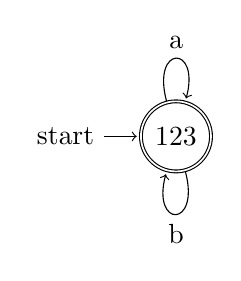
\begin{tikzpicture}[shorten >= 1pt, node distance = 2cm, on grid, auto]
  \node[state, initial, accepting] (123) {123};
  \path[->]
    (123) edge [loop above] node {a} (123)
          edge [loop below] node {b} (123);
\end{tikzpicture}

\end{document}
